%We implemented the proposed approach to open-world mission specification in LTLMoP (the Linear Temporal Logic Mission Planning toolkit; see Section \ref{preliminariesB}). We augmented Structured English, one of LTLMoP's available specification languages, with \emph{open-world abstractions} (groups, quantifiers, and correspondences), the \emph{add to group} operator, and a \emph{resynthesis} action.
We implemented the proposed approach to open-world mission specification in LTLMoP (see Section \ref{preliminariesB}). We augmented Structured English with \emph{open-world abstractions} (groups, quantifiers, and correspondences), the \emph{add to group} operator, and a \emph{resynthesis} action.

\begin{myExample}\label{Ex:mailbot3} We revisit the mailbot scenario from Examples \ref{Ex:mailbot1} and \ref{Ex:mailbot2}, and present the full mission specification, $\mathcal{M}_0$.
%The robot's workspace is depicted in Fig. \ref{Fig:map}. 
%The LTLMoP simulation is presented in Fig. \ref{Fig:sim}.
The robot's workspace can be seen in Fig. \ref{Fig:sim1}.
\end{myExample}

Initially, the robot has no information about specific letters or their recipients. Therefore, it patrols the regions in \texttt{PatrolRooms}. If it senses a new letter (see Fig. \ref{Fig:sim1}), it will add a proposition to the group \texttt{Letters}. In simulation, LTLMoP prompts the user for the name of the proposition, e.g. \texttt{letter1}. Additionally, the \emph{add to} operator has to add a proposition to the group \texttt{Offices}, in order to maintain the correspondence. LTLMoP prompts the user a second time, and the user inputs one of the region names, \texttt{r1}--\texttt{r6} (see Fig. \ref{Fig:sim2}). The two user prompts simulate the process of scanning the letter for the recipient's name and address, in order to name and ground the new propositions (see Assumption \ref{Ass:grounding}).

\begin{algorithm}
	\textbf{Mission specification:} Autonomous Mailbot
	
	\vspace{-7 pt}
	\hrulefill
	{\small
	
	\textbf{Group declarations:}\\
	\texttt{Group Letters is empty} \\
%	\texttt{Group LetterSlots is empty} \\
%	\texttt{Group Delivery is empty} \\
	\texttt{Group Offices is empty} \\
	\texttt{Group PatrolRooms is mailRoom, hallW, hallN}
	
	\textbf{Correspondence definitions:} (immutable)\\ %FIXME: Add more for add_to to work?
%	\texttt{Letters correspond to LetterSlots, Delivery, Offices}\\ %FIXME: This isn't implemented
%	\texttt{LetterSlots correspond to Letters}\\
%	\texttt{LetterSlots correspond to Delivery}\\
%	\texttt{Delivery correspond to LetterSlots}\\
%	\texttt{Delivery correspond to Offices}\\
	\texttt{Letters correspond to Offices}
	
%	\hrulefill\\
	% TODO: We can't have initial conditions when we are re-synthesizing, right?
%	\textbf{Initial conditions} (optional)\\
%	\texttt{Robot starts in mailRoom with false}\\
%	\texttt{Environment starts with false}\\
	
	\textbf{Mission tasks:} (immutable)\\
	\texttt{If you are sensing any Letters then go to the corresponding Office}\\
	\texttt{If you are not sensing any Letters then visit each PatrolRoom}
%	\texttt{Each LetterSlot is set on the corresponding Letter and pickUp and reset on the corresponding Delivery}\\
	
%	\texttt{Do pickUp if and only if you are sensing any Letters}\\
%	\texttt{If you are activating pickUp then stay there}\\
	
%	\texttt{Do each Delivery if and only if you are in the corresponding Office and you are activating the corresponding LetterSlot}\\
	
%	\texttt{Infinitely often not each LetterSlot}\\
%	\texttt{If you are not activating any LetterSlots then visit each PatrolRooms}\\
	
	\textbf{Open--World settings:} (immutable)\\
	\texttt{If you are sensing newLetter then add to group Letters and resynthesize}\\
%	\texttt{If you are sensing newLetter then stay there}\\
		
%	\textbf{Environment fairness assumption:} (immutable)\\
%	\texttt{Infinitely often not any Letters}\\
%	\texttt{Infinitely often not newLetter}\\
	}
	\vspace{-8 pt}
\end{algorithm}
\vspace{-5 pt}
%\begin{figure}[h]
%	\centering
%	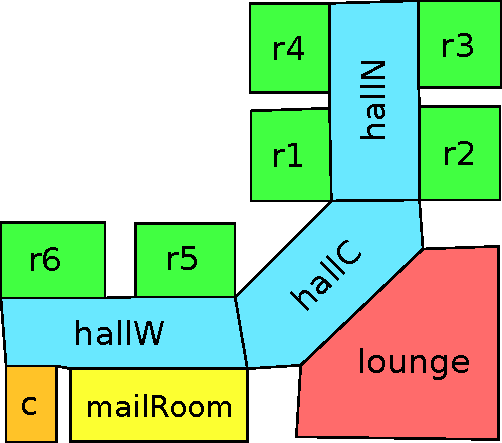
\includegraphics[width=0.70\columnwidth, clip]{./img/mailbot_map.pdf}
%	\caption{Map of workspace for mailbot scenario.  Regions \texttt{r1}--\texttt{r6} are the offices of potential letter recipients.} 
%	\label{Fig:map}
%\end{figure}

After the specification is rewritten, the LTL formula $\varphi [k]$ changes to $\varphi [k+1]$, according to Eqs. \eqref{Eq:newSpecA} and \eqref{Eq:newSpecB}. The change involves adding a new mission goal: the delivery of \texttt{letter1} to the corresponding office \texttt{r1}. Specifically, compared to $\varphi_g^s [k]$, $\varphi_g^s [k+1]$ contains the additional liveness requirement:
$\G\F\left( \texttt{letter1} \Rightarrow \texttt{r1} \right)$.

After resynthesis (see Fig. \ref{Fig:sim3}), the robot can now sense letters in two ways. First, it could detect a letter addressed to the same recipient as \texttt{letter1}. In this case, \texttt{letter1} will become \texttt{True}, and the robot will deliver the letter to \texttt{r1}. Second, it could detect a letter addressed to a new recipient. In that case, the sensor \texttt{newLetter} will become \texttt{True}, and the \emph{add to group} operator will once again cause new propositions to be added to \texttt{Letters} and \texttt{Offices}.

\begin{figure}[h]
	\centering
	\begin{subfigure}[b]{0.99\columnwidth}
	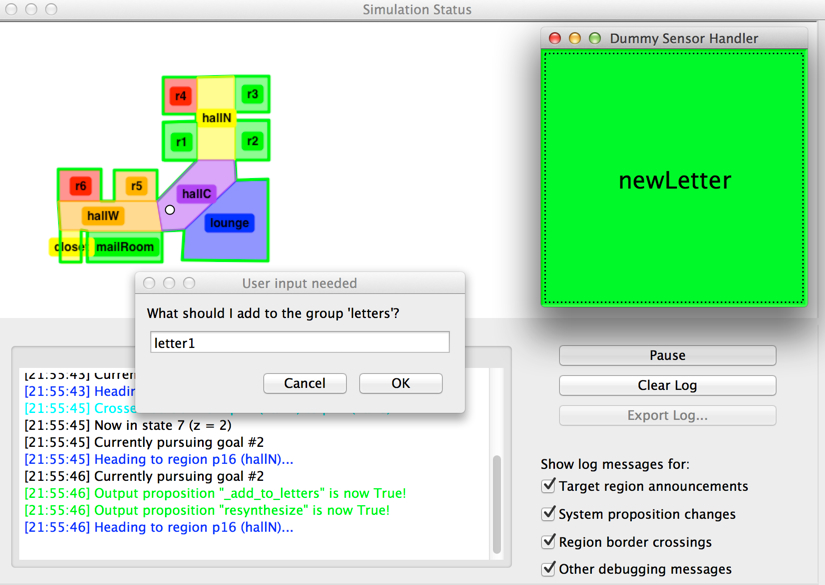
\includegraphics[width=0.99\columnwidth, clip]{./img/sim1.jpg}
	\caption{A new letter is detected. The user names the new proposition.} 
	\label{Fig:sim1}
	\end{subfigure}
	
	\vspace{4 pt}
	\begin{subfigure}[b]{0.99\columnwidth}
	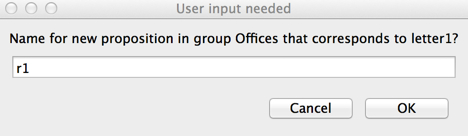
\includegraphics[width=0.99\columnwidth, clip]{./img/sim2.jpg}
%	\caption{The user grounds the corresponding office proposition.} 
%	\caption{The user grounds the corresponding office proposition, $\mathcal{C}(\texttt{letter1})$, to \texttt{r1}, one of the existing regions.} 
	\caption{The user grounds the corresponding office proposition to \texttt{r1}.} 
	\label{Fig:sim2}
	\end{subfigure}
	
	\vspace{4 pt}
	\begin{subfigure}[b]{0.99\columnwidth}
	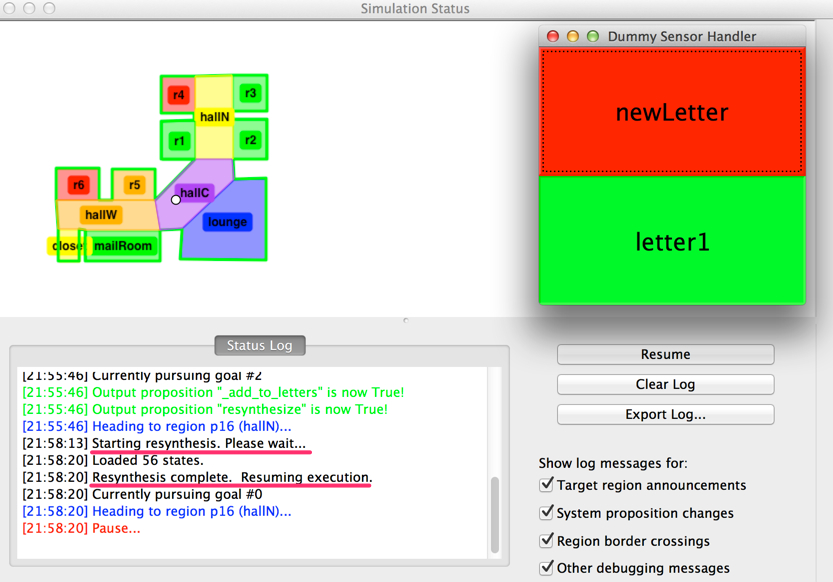
\includegraphics[width=0.99\columnwidth, clip]{./img/sim3.jpg}
%	\caption{\texttt{letter1} and \texttt{r1} were added to \texttt{Letters} and \texttt{Offices}, respectively. Execution resumes, with \texttt{letter1} = \texttt{True}.} 
	\caption{\texttt{letter1} and \texttt{r1} were added to \texttt{Letters} and \texttt{Offices}.} 
	\label{Fig:sim3}
	\end{subfigure}
	\caption{Simulation of Example \ref{Ex:mailbot3} in LTLMoP.}\label{Fig:sim}
\end{figure}

% END